\subsection{Peak Traffic Demand}\label{subsec:peakratio}

The Sandvine Reports show that although the mean usage has remained
stable for the past few years, usage during peak-times has increased
drastically~\cite{sandvine20141h}. To measure this growth, they introduce the
concept of peak period, measured when the network is within 95\% of its highest 
point. Although, these reports present a good view into aggregate usage 
patterns over a month,
they neglect to analyze usage characteristics individually. Inspired by their
definition, we measure the disparity between the 95 percentile of the peak and 
median
usage of each household within a day, and call this the \emph{Peak-Ratio}.


\begin{figure}[t]
\begin{minipage}{1\linewidth}
\centering
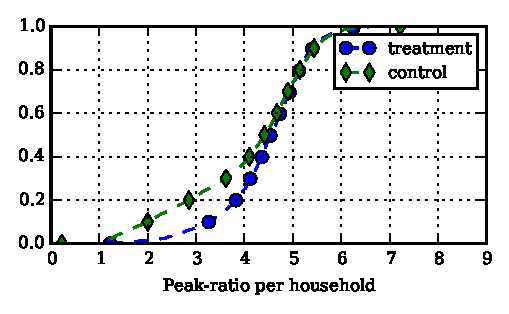
\includegraphics[width=1\linewidth]{figures/peakratio-CDF-devices-MEAN.pdf}
\caption{Distribution of peak ratio for subscribers in the treatment and 
control groups. For 40 percent of the users with most disparity between their
95 percentile and mean demand in a day, the peak-ratio stays the same due to 
the service upgrade. For 60 percent of the users with a low peak ratio in the 
control group have a higher peak ratio in the treatment group. \red{fix aspect 
ratio, not log x scale}}
\label{fig:CDF-peak-ratio-mean}
\end{minipage}
\end{figure}

Figure ~\ref{fig:CDF-peak-ratio-mean} shows that the mean peak-ratio for each 
device in the \test set is much larger than that of the \control set.
\todo{replace much larger with the exact number or percentage}.
\sg{Taken together} with our observations of a lower prime-time ratio of the  
\test set (section~\ref{subsec:primetime}) this implies that there are 
households in the \test set that achieve a peak-ratio $>$ 1, but not during the 
prime-time hour. We believe that these households might actually be small 
businesses or work-at-home users that peak during daytime hours instead of 
evening hours.

The mean peak-ratio varies between \todo{X} and \todo{Y}. There are 
some households that have a very even usage throughout the day (low peak ratio), 
and others that are extremely aggressive only at a certain times of a day (high 
peak ratio).